\chapter{Durchführung}

\section{$\alpha_p$-Studie}{Ziad}

Erwähnung von Ti64 nochmal und (TS-STDA) Three Step short Time duplex Anneal
\section{$\alpha_p$-Studie}

\section{Martensit-Bildung}{Thiago}



\section{Martensit-Bildung}

\section{Martensit-Zerfall}{Viktor}

Um Martensit zu bilden werden Ti64-Teile  nach der ersten Wärmebehandlung, wie es in Abbildung \ref{STDA} zusammengefasst wird, für 1 min  bei 930°C erwärmt und dann  auf Raumtemperatur wassergekühlt. Unter dem Einfluss von der Diffusion soll sich die erhaltene und metastabile Beta Phase aus der bimodalen Struktur weiter wachsen. Die kurze Erwärmungszeit soll dafür sorgen, dass die neu gebildeten Beta-Gebiete nicht mit $\beta$-Stabilisatoren, in diesem Fall Vanadium, bereichert  und dadurch stabilisiert werden. Durch das schnelle Abschrecken auf Raumtemperatur wandelt sich das "neue "$\beta$ diffusionslos und lokal in Martensit um. 

\begin{figure}[H]
	\centering
	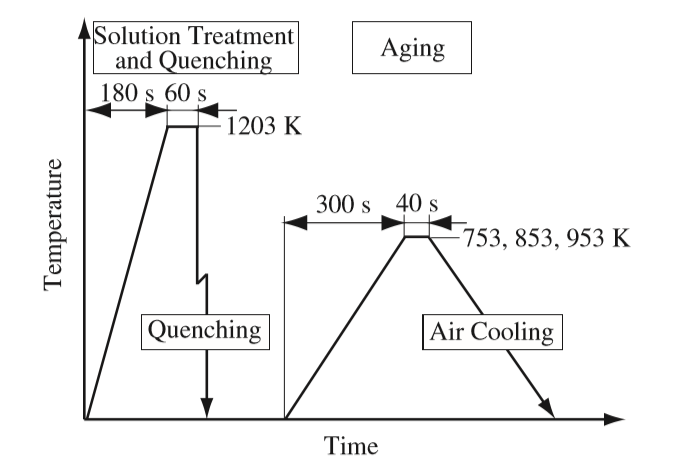
\includegraphics[width=0.9\textwidth]{Bilder/ts-stda}
	\caption{Vorgehensweise nach dem Duplex-Anneal bei STDA für Ti-64 (Strengthening of Ti–6Al–4V Alloy by Short-Time Duplex Heat Treatment)}
	\label{STDA}
\end{figure}

Da die $\beta_{t}$ von Ti-64 relativ niedriger ist als die von Ti-6242, liegt auch ihrer Gleichgewichtstemperatur unterhalb der von Ti-6242. Außerdem hat Vanadium im Vergleich zu Molybdän eine viel größere Diffusionsrate in Titan, was die schnellen Anlasszeiten noch weiter erklärt[Titan und Titan legierungen, Zwicker]. Aus diesen Gründen wurden in diesem Schritt die Ti-6242-Proben nach dem Duplex-Anneal für 8-16 min jeweils bei 930°C und 950°C wärmebehandelt.

Eine bekannte Wärmebehandlung von $\alpha$+$\beta$-Titanlegierungen ist die  \textit{Solution treatment and quenching}, wobei die Titanlegierung direkt von einer Temperatur $T_{1}$ unterhalb  $\beta_{t}$ nach 0,5-1 h abgeschreckt wird. Wie bei der oben beschriebenen Wärmebehandlung stellt sich bei $T_{1}$ ein zweiphasiges Gefüge mit $\alpha_p$ und $\beta$ ein. Die $\beta$-Phase wandelt sich  dann auch beim Abschrecken martensitisch um und wird $\alpha^\prime$ genannt.
Zum Vergleich zu der studierten Wärmebehandlung werden AR-Proben bei 983°C für 1h erwärmt und wassergekühlt.

\section{Martensit-Zerfall}